
Gestures are classified into static gestures and dynamic gestures. Group of static gestures consits of fixed gestures which are not relative to time, where group of dynamic gestures are time varying.

Hand and body gesture recognition had followed a conventional scheme of extracting key features via one or multiple preprocessing sensors and applying machine learning techniques on them.\cite{avola}

\section{Tracking devices}
The field of gesture recognition gave birth to several image processing devices yielding useful data. 
\subsection{Microsoft Kinect}
%=======================================================================================================================
One of them being Micorosoft Kinect, a device first released in 2010. Originaly developed for gaming but eventually finding more success in academics and commercial applications, such as robotics, medicine, and health care. Leading Microsoft to discontinue production of its Xbox version in 2018 and releasing Azure Kinect in March 2020, incorporating Microsoft Azure cloud computing funcitionalities.

\begin{figure}[ht]
	\centering
    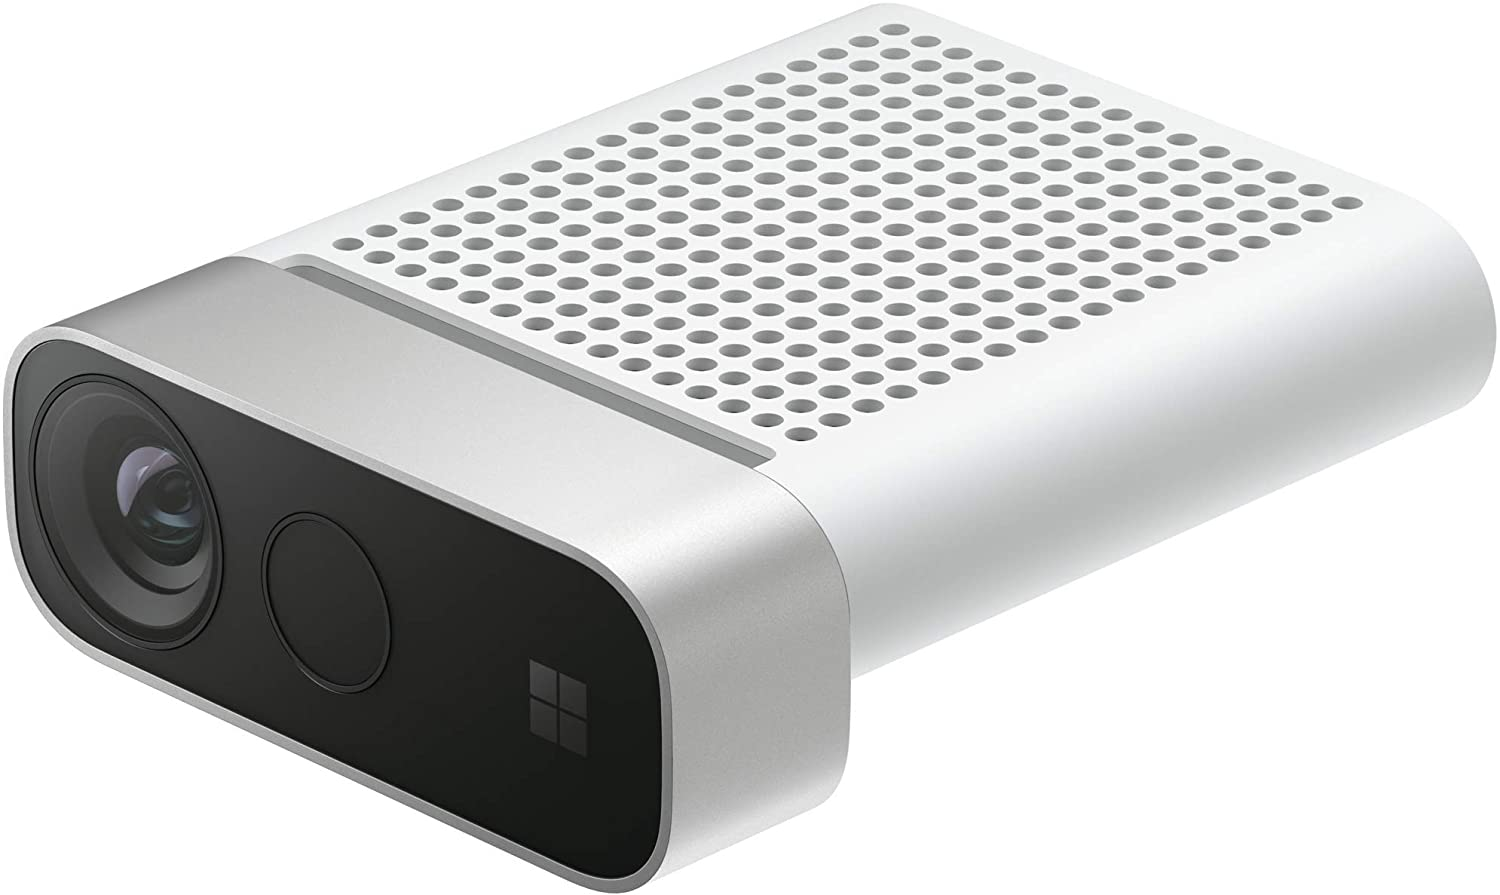
\includegraphics[width=8cm]{azure_kinect.jpg}
	\caption{Azure Kinect \cite{azurekinect_pic}}
	\label{fig:azureKincet}
\end{figure}

Azure Kinect contains a depth sensor, spatial microphone array with a video camera, and orientation sensor as an all in-one small device with multiple modes, options, and software development kits.\cite{azurekinect}

With all that said main purpose of the Kinect device overall is to interpret whole-body movement. For such it is lacking in required accuracy for hand gesture recognition. 

\subsection{Leap Motion Controller}
%=======================================================================================================================

Another option would be using a Leap Motion Controller (LMC), developed specifically to track hand movements and extract its features, such as positions of fingers, hand rotation, and others.

LMC consists of two monochromatic IR cameras and three IR LEDs (emitters). 

\begin{figure}[h]
	\centering
    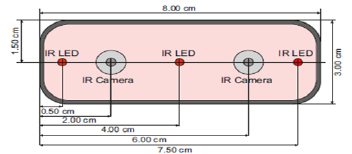
\includegraphics[width=8cm]{lmc_schematic.png}
	\caption{Schematic View of Leap Motion Controller}
	\label{fig:lmcScheme}
\end{figure}



The LMC's current API, Leap Motion Service, yields positions of extracted hand features. All the positional data about the hand and its features are represented in the coordinate system relative to the LMC's center point, positioned at the middle IR LED.\cite{LMCanalysis} The x- and z-axes lie in the camera sensors plane, with the x-axis running along the camera baseline. The y-axis is vertical, with positive values increasing upwards (in contrast to the downward orientation of most computer graphics coordinate systems). The z-axis has positive values increasing toward the user.\cite{tomasMultileap}

\begin{figure}[H]
	\centering
    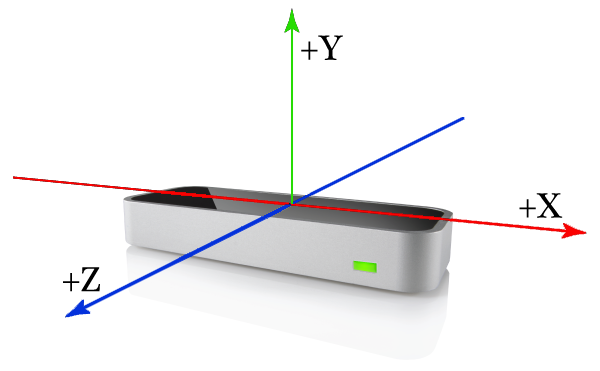
\includegraphics[width=8cm]{leap_axes.png}
	\caption{Leap Motion Controller Axes}
	\label{fig:lmcScheme}
\end{figure}

Unfortunately, Leap Motion Controller has no official library for gesture recognition, limiting developers from utilizing the controller for its key features. Leap Motion provided tracking software built for virtual reality, used to have a gesture detector with its 3.0 version, but the detector is absent with the release of more accurate version 4.0.

\subsection{Ultraleap Stereo IR 170}

Ultraleap Stereo IR 170, formerly known as the Leap Motion Rigel, is the successor to the Leap Motion controller.

The Ultraleap inherits Leap Motions key features, but improves with wider 170-degree field of view, more-powerful LED illuminators providing longer tracking range, and a higher framerate when used with USB 3.0.\cite{ultraleap}\cite{ultraleap2}

\begin{figure}[h]
	\centering
    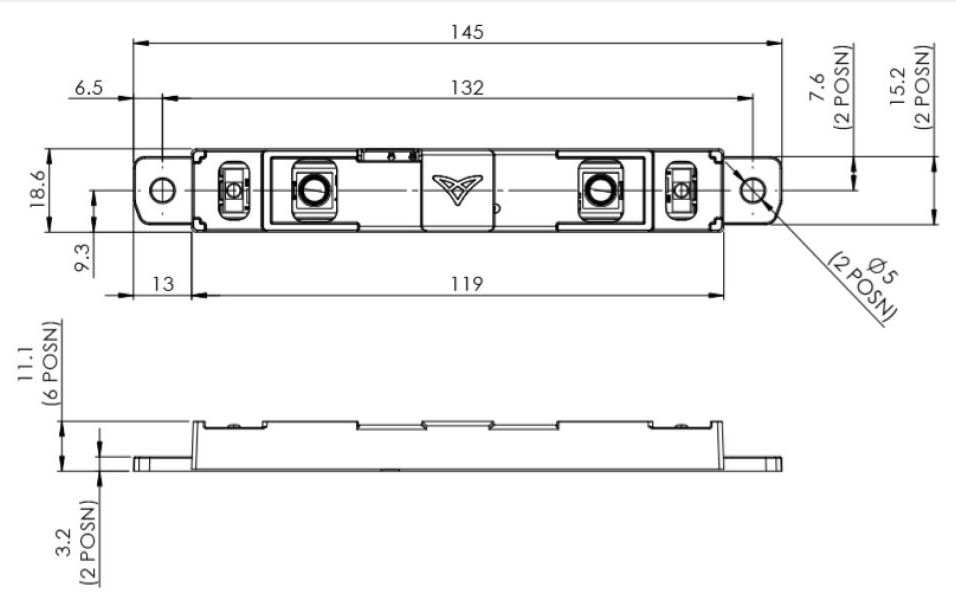
\includegraphics[width=8cm]{ultraleap_pic.jpg}
	\caption{Schematic View of Ultraleap Stereo IR 170 \cite{ultraleap}}
	\label{fig:lmcScheme}
\end{figure}



\section{Gesture Recognition Methods
}
%=======================================================================================================================

Gestures classification should be taken into account when choosing appropriate methods due to their time-varying properties. As previously mentioned, gestures are classified into static and dynamic groups.

\subsection{Static Gesture Recognition}

One of the commonly used method for static gesture recognition are \textit{Support Vector Machine} (SVM), an algorithm used for both regresseion and classification tasks alike. But overall, it is widely used in classifications. SVM's goal is to find a \textit{hyperplane} in N-dimension space, N being the number of features, that distictivly classifies data points.\cite{svmIntroToML} 
\textit{Hyperplanes} are decision boundaries between data points and optimal \textit{hyperplane} is the one with maximal seperation, \textit{margin}, between classes.
Vector Machines (SVM). , ANN, or pattern techniques.\cite{savaris}.

Chen and Tseng \cite{chentseng} presented an SVM solution for multi-angle hand gesture recognition for rock paper sissors using images from webcamera. The trainning dataset consisted of 420 images and testing set of 120 images. 
Datasets were collected from 5 different people for the right hand only and achieving 95\%. The classifier still managed to recognize left hand gestures with 90\% accuracy. 

Domino et al. \cite{dominokinect} utilized SVM with Microsoft Kinect sensors. Extracting hand features, finger tips and center of the hand, from depth map and feading the data into SVM. Achieving 99.5\% recognition rate on dataset provided by Ren et Al. \cite{dominokinect_data} The dataset consists of 10 different gestures performed by 10 different people repeatedly each 10 times, total of 1000 different depth maps.

Mapari and Kharat\cite{mapari} on the other hand proposed a method to recognize American Sign Language (ASL) with an \textit{Feed-forward network} using \textit{Multilayer Perceptron (MLP)}, extracting data from LMC and computing 48 features (18 positional values, 15 distance values, and 15 angle values) for 4672 collected signs (146 users for 32 signs). The average classification accuracy is 90\%.

\subsection{Dynamic Gesture Recognition}

Katia et al. \cite{katiacnn} proposed a method classifying dynamic gestures acquired through LMC with a CNN.
Adopting a modified version of ResNet-50 architecture, a 50 layers deep CNN, by removing the last fully connected layer and adding a new layer with as many neurons as the considered collection of gesture classes. 
The acquired gesture information is converted into hand joints color images, where the variation of hand joint positions during the gesture are projected on a plane and temporal information is represented with color intensity of the projected points. Trained model achieved 91\% classification accuracy on the LMDHG dataset.\cite{lmdhg}

Yang L., Chen J. and Zhu W. \cite{bidirect_dynam} used two-layer Bidirectional RNN in combination with an LMC to classify dynamic hand gestures represeted by sets of feature vectors (finger tip distance, angle, height, the angle of adjacent fingertips and the coordinates of the palm). The proposed method has been tested on the American Sign Language (ASL) datasets with 360 samples and Handicraft‐Gesture dataset with 480 samples, achieving 90\% and 92\% accuracy.\cite{bidirect_dynam}

Ameur et al. \cite{ameur} presented a solution using SVM classifier used with LMC acquired data, (X,Y,Z) coordinates of fingertips and palm center. The experimental results show accuracy of 81\% on dataset containing 11 actions, performed by 10 different subjects, having in total 550 samples.



% \subsection{LSTM}
% Many of the proposed methods focus either on static gesture recognition or dynamic gesture recognition, but very few of them are actually utilized for both types at the same time. 